\section{Выполнение задания}

Работа выполнена на языке \verb|C++14|.

Для тестирования блокировки был реализован класс \verb|TestLock|.
\verb|TestLock| запускает несколько потоков, вызывающих определённую функцию.

Входные параметры:

\begin{itemize}
    \item \verb|name| -- Имя блокировки (отображается в логах);
    \item \verb|spins| -- Количесво выполнений для нагрузочной функции (по умолчанию = 32768);
    \item \verb|start| -- Стартовое количество потоков (по умолчанию = 1);
    \item \verb|end| -- Конечное количество потоков (по умолчанию = максимальному количеству потоков на процессоре);
    \item \verb|job| -- Нагрузочная функция (по умолчанию = TestLock::spinner).
\end{itemize}

В цикле \verb|TestLock| запускает $ (start, start + 1, \dots, end) $ потоков
на нагрузочной функции и замеряет время выполнения. 
Результаты записываются в ассоциативный массив пар 
(кол-во потоков : время выполнения)
и возвращаются на выходе.

Тестирование проводилось на \verb|CPU| модели\\
\verb|AMD Ryzen 3 3200U with Radeon Vega Mobile Gfx|
c 4 \verb|CPUs|.

\subsection*{Тест (spins=4096)}

Результаты тестирования представленны в таблице \ref{tab:results4096}


\begin{table}[H]
    \centering
    \begin{tabular}{|l|l|}
        \hline
        Кол-во потоков & Время выполнения (мс) \\
        \hline
        1 & 0 \\
        \hline
        2 & 1 \\
        \hline
        3 & 1 \\
        \hline
        4 & 5 \\
        \hline
    \end{tabular}
    \caption{Результаты тестирования для spins=4096}
    \label{tab:results4096}
\end{table}
        

График результатов тестирования представлен на рис.\ref{fig:plot4096}

\begin{figure}[H]
    \centering
    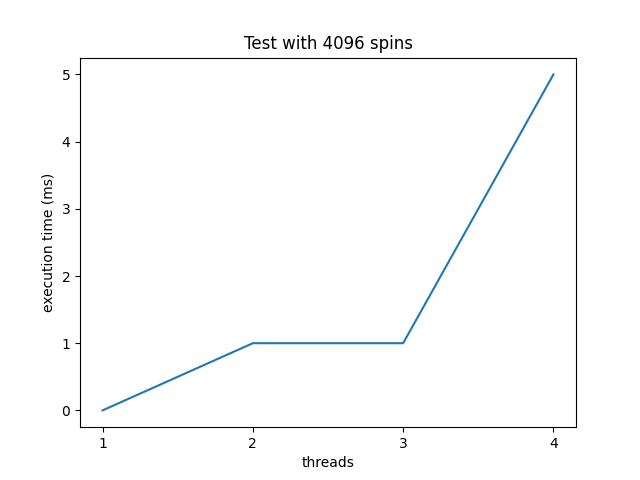
\includegraphics[width=0.7\linewidth]{photo/plot4096}
    \caption{График результатов тестирования для spins=4096}
    \label{fig:plot4096}
\end{figure}

\subsection*{Тест (spins=32768)}

Результаты тестирования представленны в таблице \ref{tab:results32768}


\begin{table}[H]
    \centering
    \begin{tabular}{|l|l|}
        \hline
        Кол-во потоков & Время выполнения (мс) \\
        \hline
        1 & 2 \\
        \hline
        2 & 18 \\
        \hline
        3 & 4 \\
        \hline
        4 & 10 \\
        \hline
    \end{tabular}
    \caption{Результаты тестирования для spins=32768}
    \label{tab:results32768}
\end{table}
        

График результатов тестирования представлен на рис.\ref{fig:plot32768}

\begin{figure}[H]
    \centering
    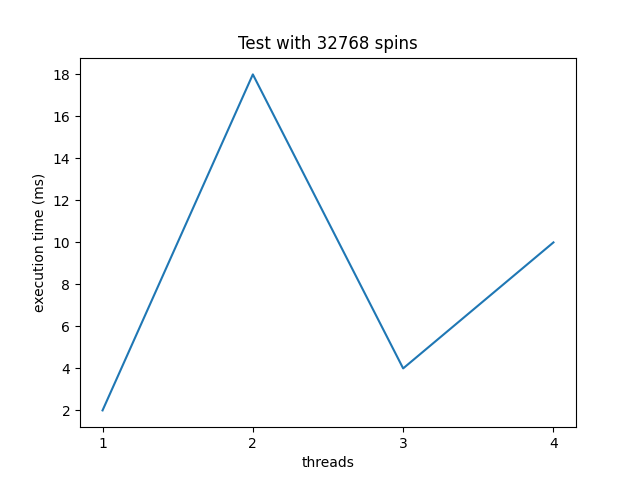
\includegraphics[width=0.7\linewidth]{photo/plot32768}
    \caption{График результатов тестирования для spins=32768}
    \label{fig:plot32768}
\end{figure}

\subsection*{Тест (spins=131072)}

Результаты тестирования представленны в таблице \ref{tab:results131072}


\begin{table}[H]
    \centering
    \begin{tabular}{|l|l|}
        \hline
        Кол-во потоков & Время выполнения (мс) \\
        \hline
        1 & 6 \\
        \hline
        2 & 17 \\
        \hline
        3 & 94 \\
        \hline
        4 & 224 \\
        \hline
    \end{tabular}
    \caption{Результаты тестирования для spins=131072}
    \label{tab:results131072}
\end{table}
        

График результатов тестирования представлен на рис.\ref{fig:plot131072}

\begin{figure}[H]
    \centering
    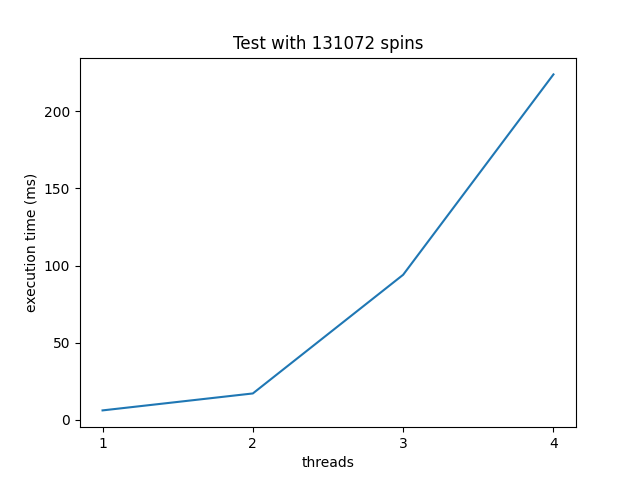
\includegraphics[width=0.7\linewidth]{photo/plot131072}
    \caption{График результатов тестирования для spins=131072}
    \label{fig:plot131072}
\end{figure}

\subsection*{Тест (spins=524288)}

Результаты тестирования представленны в таблице \ref{tab:results524288}


\begin{table}[H]
    \centering
    \begin{tabular}{|l|l|}
        \hline
        Кол-во потоков & Время выполнения (мс) \\
        \hline
        1 & 26 \\
        \hline
        2 & 101 \\
        \hline
        3 & 274 \\
        \hline
        4 & 380 \\
        \hline
    \end{tabular}
    \caption{Результаты тестирования для spins=524288}
    \label{tab:results524288}
\end{table}
        

График результатов тестирования представлен на рис.\ref{fig:plot524288}

\begin{figure}[H]
    \centering
    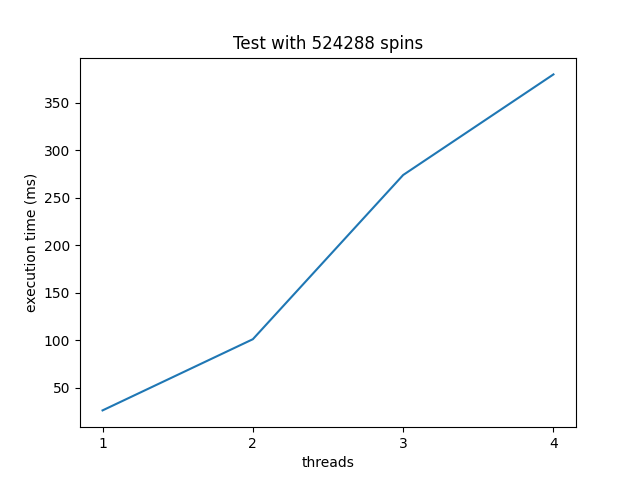
\includegraphics[width=0.7\linewidth]{photo/plot524288}
    \caption{График результатов тестирования для spins=524288}
    \label{fig:plot524288}
\end{figure}

\subsection*{Усреднённые результаты тестирования}

Усреднённые результаты тестирования представленны в таблице \ref{tab:results_mid}


\begin{table}[H]
    \centering
    \begin{tabular}{|l|l|}
        \hline
        Кол-во потоков & Время выполнения (мс) \\
        \hline
        1 & 8 \\
        \hline
        2 & 34 \\
        \hline
        3 & 93 \\
        \hline
        4 & 154 \\
        \hline
    \end{tabular}
    \caption{Усреднённые результаты тестирования}
    \label{tab:results_mid}
\end{table}
        

График усреднённых результатов тестирования представлен на рис.\ref{fig:plot_mid}

\begin{figure}[H]
    \centering
    \begin{subfigure}[b]{0.45\textwidth}
        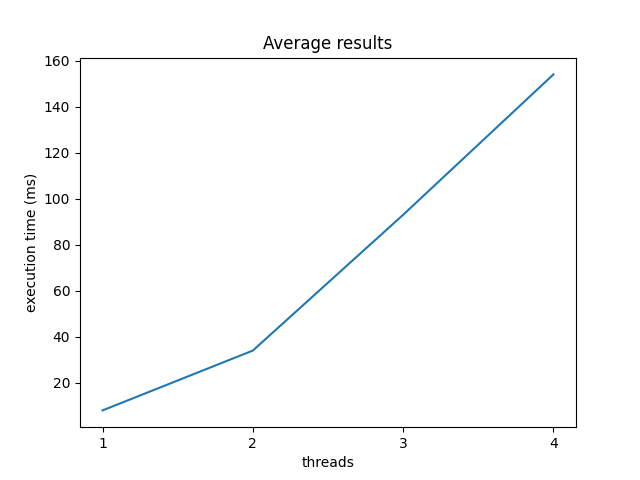
\includegraphics[width=\linewidth]{photo/plot_mid}
        \caption{График усреднённых результатов тестирования}
        \label{fig:plot_mid}
    \end{subfigure}
    \hfill
    \begin{subfigure}[b]{0.45\textwidth}
        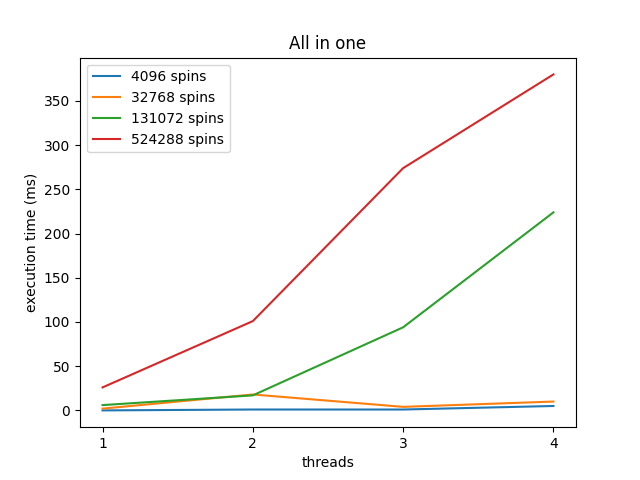
\includegraphics[width=\linewidth]{photo/all_in_one}
        \caption{Графики результатов тестирования}
        \label{fig:all_in_one}
    \end{subfigure}
    \caption{Графики результатов тестирования}
\end{figure}
